\section{Стохастическая модель}

    \subsection{Описание вносимого возмущения}

        После завершения детерминированного анализа можно перейти к стохастическому анализу. В модели (\ref{origin}) появляется слагаемое, которое отвечает за случайные возмущения. Оно имеет следующий вид: \(\varepsilon \xi\), где \(\varepsilon\) --- интенсивность шума, а \(\xi\) --- нормальная случайная величина. Это слагаемое может быть внесено аддитивно в правую часть уравнения или же в параметр модели. 
        
        Каждый вид шума несет свой биологический смысл. Например, увеличение численности популяции может происходить неравномерно из-за внешних обстоятельств, такому поведению системы соответствует \(\alpha\)-шум. \(\beta\)-шум показывает, что среда обитания также может в зависимости от времени предоставлять разное количество ресурсов для поддержания численности популяции. И наконец, аддитивный шум показывает, что рассматриваемая среда обитания необязательно должна быть изолирована от окружающего мира, может наблюдаться миграция особей.
        
        Отображения для разных видов шума примет формы, которые перечислены ниже.

        \begin{enumerate}
            \item \(\alpha\)-шум

                \begin{equation}
                    \label{alpha_chaos}
                    x_{t + 1} = \frac{(\alpha + \varepsilon \xi) x_t^2}{(\beta + x_t)^6}
                \end{equation}
    
            \item \(\beta\)-шум
    
                \begin{equation}
                    \label{beta_chaos}
                    x_{t + 1} = \frac{\alpha x_t^2}{(\beta + \varepsilon \xi + x_t)^6}
                \end{equation}
    
            \item Аддитивный шум
    
                \begin{equation}
                    \label{additive_chaos}
                    x_{t + 1} = \frac{\alpha x_t^2}{(\beta + x_t)^6} + \varepsilon \xi
                \end{equation}
        \end{enumerate}

    \subsection{Временные ряды}

        На временных рядах можно продемонстрировать как различные виды шума влияют на поведение системы.

        На рисунке \ref{time_series_x_0_06_a_1_b_0_56} изображено поведение модели без добавления каких-либо шумов. Видно, что значения переменной \(x\) с течением времени стабилизируются. Численность популяции фактически остается неизменной.

        \begin{figure}
            \centering
            \subfloat[Для модели (\ref{origin})]{
                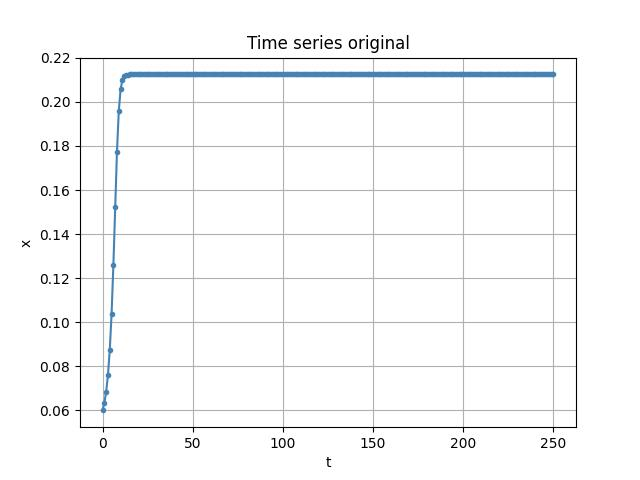
\includegraphics[width=0.5\textwidth]{stochastic/time_series_x_0_06_a_1_b_0_56.jpg}
                \label{time_series_x_0_06_a_1_b_0_56}
            }
            \subfloat[Для модели (\ref{alpha_chaos})]{
                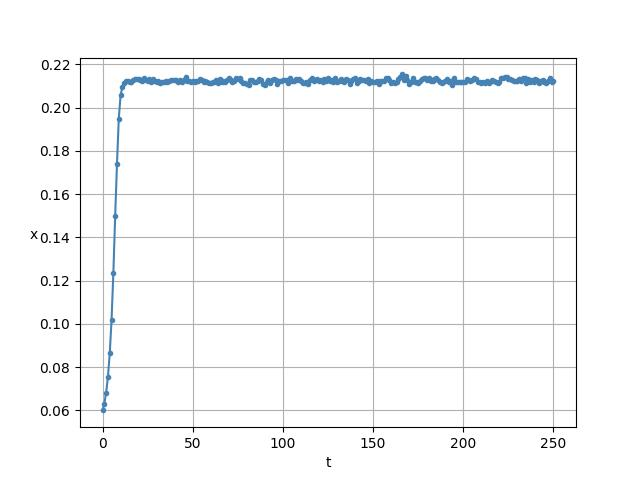
\includegraphics[width=0.5\textwidth]{stochastic/time_series_x_0_06_a_1_b_0_56_alpha_chaos_epsilon_0_004.jpg}
                \label{time_series_x_0_06_a_1_b_0_56_alpha_chaos_epsilon_0_004}
            }  

            \subfloat[Для модели (\ref{beta_chaos})]{
                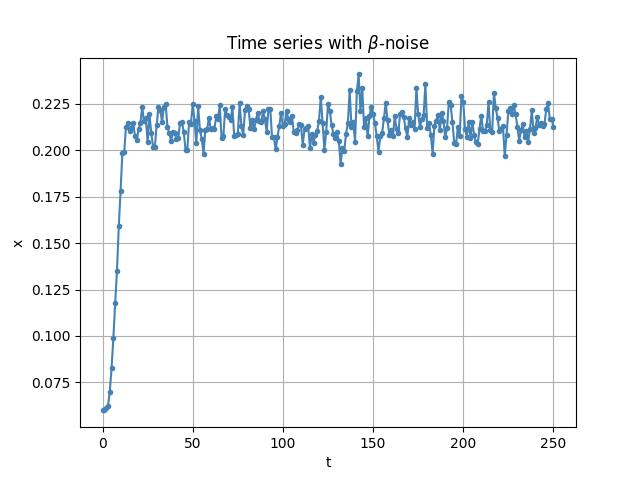
\includegraphics[width=0.5\textwidth]{stochastic/time_series_x_0_06_a_1_b_0_56_beta_chaos_epsilon_0_004.jpg}
                \label{time_series_x_0_06_a_1_b_0_56_beta_chaos_epsilon_0_004}
            }
            \subfloat[Для модели (\ref{additive_chaos})]{
                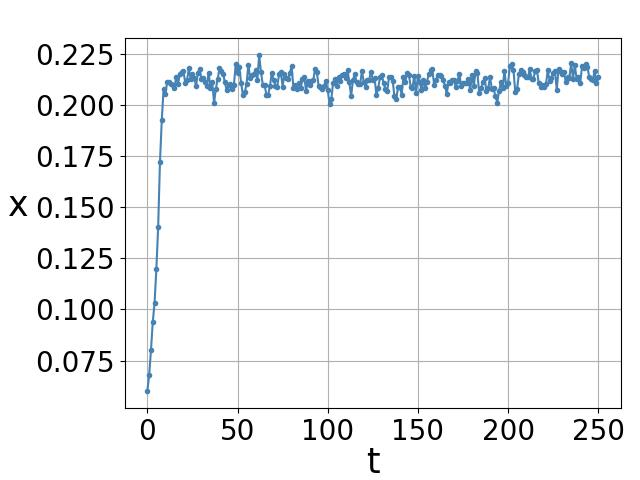
\includegraphics[width=0.5\textwidth]{stochastic/time_series_x_0_06_a_1_b_0_56_additive_chaos_epsilon_0_004.jpg}
                \label{time_series_x_0_06_a_1_b_0_56_additive_chaos_epsilon_0_004}
            }
            
            \caption{Временные ряды при \(\alpha = 1, \beta = 0.56, x_0 = 0.06, \varepsilon = 0.004\)}
        \end{figure}

        Далее на рисунках \ref{time_series_x_0_06_a_1_b_0_56_alpha_chaos_epsilon_0_004}, \ref{time_series_x_0_06_a_1_b_0_56_beta_chaos_epsilon_0_004}, \ref{time_series_x_0_06_a_1_b_0_56_additive_chaos_epsilon_0_004} представлены временные ряды для различных видов шума: 

        \begin{enumerate}[a)]
            \setcounter{enumi}{1}
            \item \(\alpha\)-шум
            \item \(\beta\)-шум
            \item аддитивный шум
        \end{enumerate}

        Все варианты рассматриваются с одной и той же интенсивностью шума \(\varepsilon = 0.004\). 
        
        Мы видим, что вид шума влияет на величину разброса значений численности популяции. \comment{Приплети сюда дисперсию.} И если раньше численность популяции стабилизировалась и переставала хоть сколько-нибудь меняться, то сейчас численность постоянно всегда колеблется, но как можно заметить, она меняется в рамках некоторого коридора значений. Численность популяции в общем то не растет и не уменьшается на какую-то значительную величину. Но такое поведение наблюдается не всегда.

        \comment{малый шум будет оказывать незначительное влияние, а большой - огромное.}

        \comment{Можно взять оригинальный временной ряд и на него сверху наложить временной ряд с шумом.}

        \comment{Хорошая фраза: индуцированный шумом переход}

        Для того чтоб продемонстрировать другое возможное поведение, давайте увеличим интенсивность шума. Пускай теперь \(\varepsilon = 0.04\). Рассмотрим рисунок \ref{time_series_x_0_06_a_1_b_0_56_beta_chaos_epsilon_0_04_fall}. Здесь мы видим ситуацию, когда шум оказал негативное влияние на численность популяции. Но опять же все не так просто. Если мы еще раз запустим алгоритм, который просчитывает нашу модель, то мы увидим, что популяция успешно выживала на протяжении анализируемого интервала времени. Данный пример проиллюстрирован на картинке \ref{time_series_x_0_06_a_1_b_0_56_beta_chaos_epsilon_0_04_alive}. Аналогичные эффекты можно наблюдать и при других видах шума.

        \comment{Примерно в \(t = 50\) обе популяции были близки к вымиранию, но одна выжила, а вторая нет. "Одно рисовое зернышко может склонить чашу весов" (с) какой-то мультик.}

        \begin{figure}
            \centering
            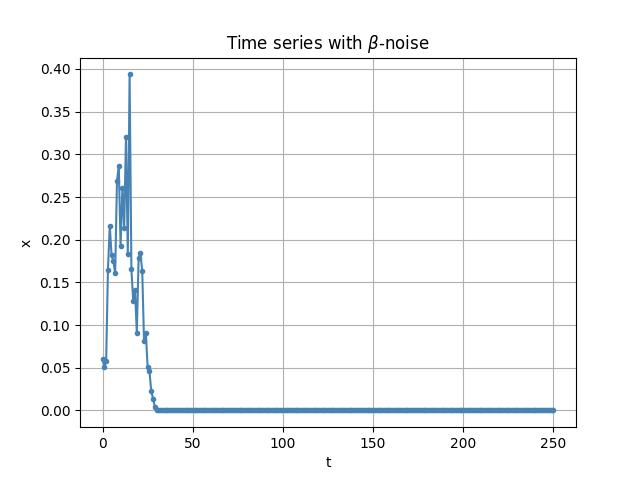
\includegraphics[width=\textwidth]{stochastic/time_series_x_0_06_a_1_b_0_56_beta_chaos_epsilon_0_04_fall.jpg}
        
            \captionsetup{justification=centering}
            \caption{Временной ряд модели (\ref{beta_chaos}) при \(\beta = 0.56, \alpha = 1, x_0 = 0.06, \varepsilon = 0.04\)}
            \label{time_series_x_0_06_a_1_b_0_56_beta_chaos_epsilon_0_04_fall}
        \end{figure}

        \begin{figure}
            \centering
            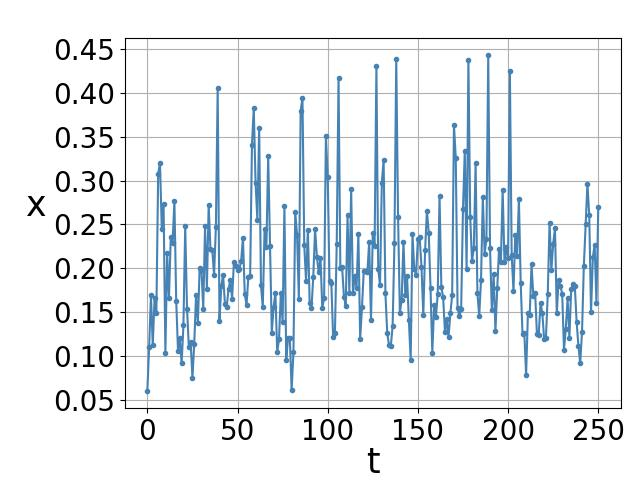
\includegraphics[width=\textwidth]{stochastic/time_series_x_0_06_a_1_b_0_56_beta_chaos_epsilon_0_04_alive.jpg}
        
            \captionsetup{justification=centering}
            \caption{Временной ряд модели (\ref{beta_chaos}) при \(\beta = 0.56, \alpha = 1, x_0 = 0.06, \varepsilon = 0.04\)}
            \label{time_series_x_0_06_a_1_b_0_56_beta_chaos_epsilon_0_04_alive}
        \end{figure}

        Анализируя вышесказанное можно сказать, что при добавлении в модель случайных событий ее поведение становится непредсказуемым. Одно незначительное изменение может кардинально повлиять на ход развития событий. 

        \comment{рассматривать как в том семестре все возможные варианты поведения системы в зависимости от начальной точки думаю не надо и так все понятно.}

    \subsection{Бифуркационные диаграммы}

        Теперь перейдем к рассмотрению графиков бифуркации моделей с разными видами шумов. На рисунках \ref{bifurcation_x_0_2_a_1_compare_beta_noise}, \ref{bifurcation_x_0_2_a_1_compare_alpha_noise} и \ref{bifurcation_x_0_2_a_1_compare_additional_noise} представлены графики бифуркационных диаграмм для моделей с \(\beta\)-шумом, \(\alpha\)-шумом и аддитивным шумом при параметре \(\beta = 1\). Эти графики похожи на детерминированный случай \ref{bifurcation_x_0_2_a_1_compare_no_noise}. На каждом графике, также как и в исходной модели, существует учсток равновесия, участки с циклами. От вида и интенсивности шума зависит то, насколько сильно отличается график с шумом относительно графика для исходной модели \ref{origin}. 

        Самое сильное влияние на значения оказывает \(\beta\)-шум. А, например, \(\alpha\)-шум оказывает незначительное влияние и график очень похож на детерминированный случай. Данные выводы также подтверждаются результатами, которые мы получили при построении временных рядов.

        \comment{Не понятно про что тут писать. Вроде про все сказали в том семетре.}

        \begin{figure}
            \centering
            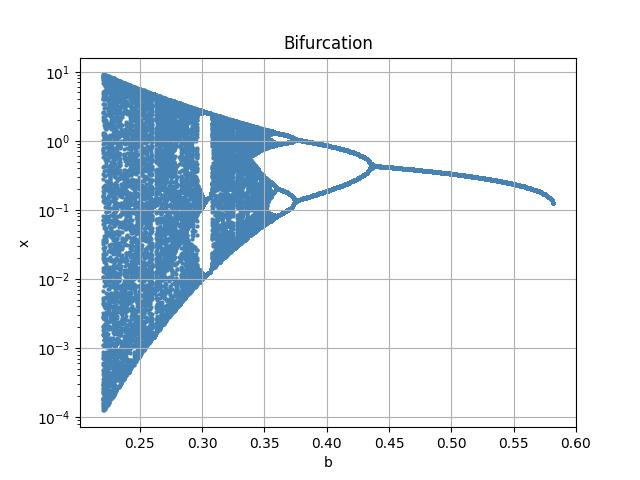
\includegraphics[width=\textwidth]{stochastic/bifurcation_x_0_2_a_1_compare_no_noise.jpg}
        
            \captionsetup{justification=centering}
            \caption{График бифуркации без шума}
            \label{bifurcation_x_0_2_a_1_compare_no_noise}
        \end{figure}

        \begin{figure}
            \centering
            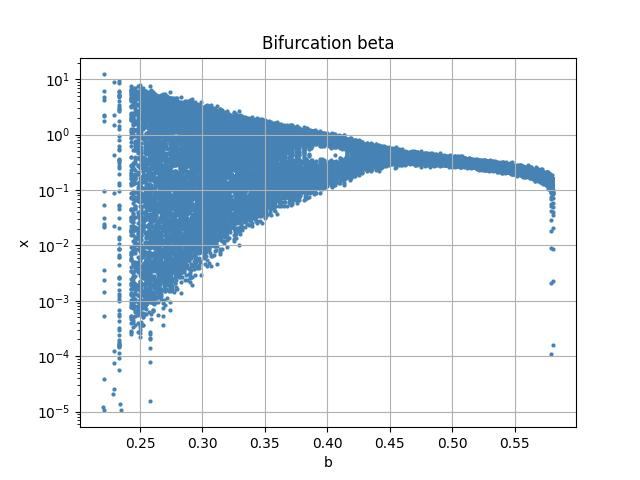
\includegraphics[width=\textwidth]{stochastic/bifurcation_x_0_2_a_1_compare_beta_noise.jpg}
        
            \captionsetup{justification=centering}
            \caption{График бифуркации с \(\beta\)-шумом, \(\varepsilon = 0.01\)}
            \label{bifurcation_x_0_2_a_1_compare_beta_noise}
        \end{figure}

        \begin{figure}
            \centering
            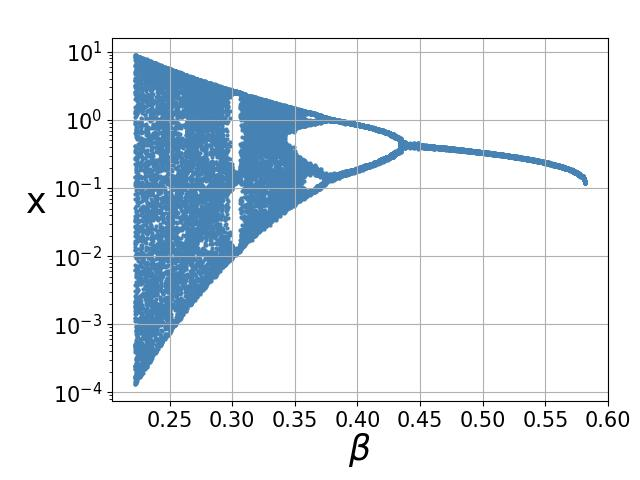
\includegraphics[width=\textwidth]{stochastic/bifurcation_x_0_2_a_1_compare_alpha_noise.jpg}
        
            \captionsetup{justification=centering}
            \caption{График бифуркации с \(\alpha\)-шумом, \(\varepsilon = 0.01\)}
            \label{bifurcation_x_0_2_a_1_compare_alpha_noise}
        \end{figure}

        \begin{figure}
            \centering
            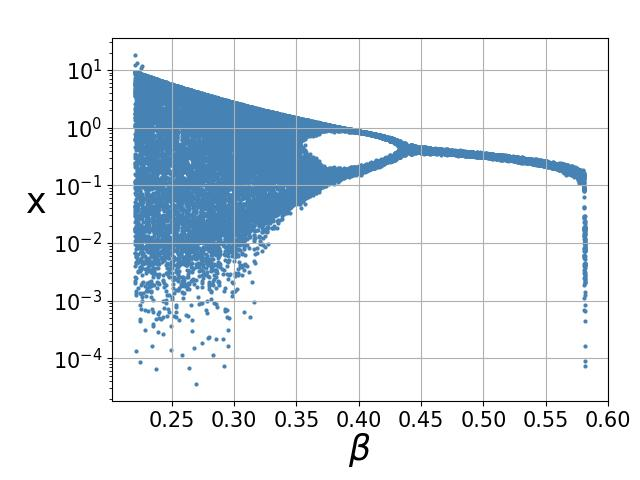
\includegraphics[width=\textwidth]{stochastic/bifurcation_x_0_2_a_1_compare_additional_noise.jpg}
        
            \captionsetup{justification=centering}
            \caption{График бифуркации с аддитивным шумом, \(\varepsilon - 0.01\)}
            \label{bifurcation_x_0_2_a_1_compare_additional_noise}
        \end{figure}

    \subsection{Матожидание}

        \comment{Напиши что-нибудь про матожидание и циклическое матожидание}

        Давайте рассмотрим график матожидания \ref{EV} для модели с \(\beta\)-шумом, которая представлена формулой \ref{beta_chaos}. Мы видим, что на графике есть "выбросы" значений, например, такое можно увидеть на черной линии в точках \(\beta = 0.38\) и \(\beta = 0.45\). Для того, чтобы избавиться от таких выбросов и получить общую картинку происходящего далее будем анализировать усредненные матожидания.

        \comment{Думаю расписывать как построили усредненное матожидание не надо.}
        
        \begin{figure}
            \centering
            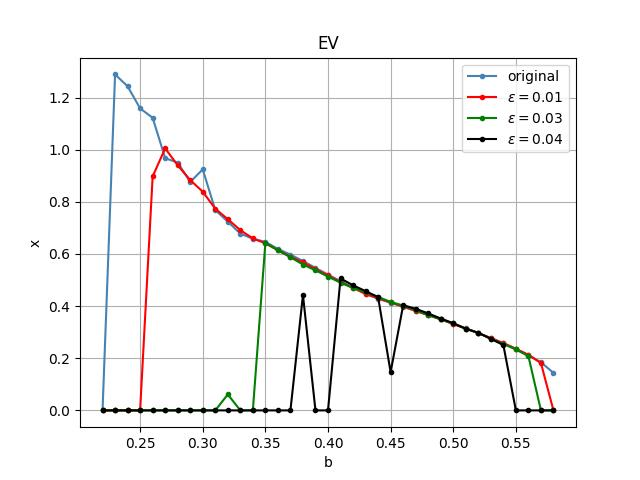
\includegraphics[width=\textwidth]{stochastic/EV.jpg}
        
            \captionsetup{justification=centering}
            \caption{}
            \label{EV}
        \end{figure}

        Перейдем к рассмотрению графика \ref{EV_cyclic} усредненных значений математического ожидния. Мы видим, что нам удалось избавиться от "выборосов", описанных выше. При этом можно оценить \comment{что происходит на участкх, которые уходят вниз.}
        
        \begin{figure}
            \centering
            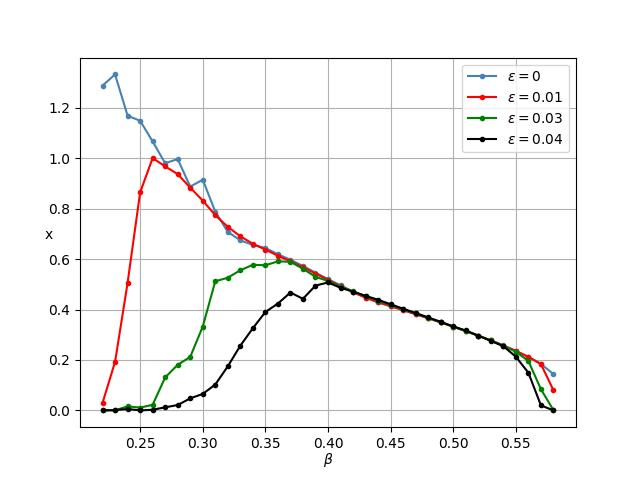
\includegraphics[width=\textwidth]{stochastic/EV_cyclic.jpg}
        
            \captionsetup{justification=centering}
            \caption{}
            \label{EV_cyclic}
        \end{figure}

        На графике матожидания видно, что значения бифуркации при уменьшении параметра \(\beta\) растет, доходит до какого-то значения и сваливается в ноль. Заметим также, что при увеличении интенсивности наша модель начинает уходить в ноль при более больших значениях параметра \(\beta\). Это связано с тем, что при более высокой интенсивноти, шум оказывает более сильное влияние на развитие популяции.

        \comment{При чем, если есть шум, то уходим в ноль всегда, а при остуствии шума начинается зона хаоса}

        \comment{Точка начала сваливания в ноль обусловлена траекториями...}

        \comment{Теперь про касания...}

        \comment{А разные шумы?}

    \subsection{Дисперсия}

        Для дисперсии будем строить усредненный график, аналогично тому, как мы сделали в пункте про матожидание.

        \comment{напиши что-нибудь про дисперсию и циклическую дисперсию}
        
        \begin{figure}
            \centering
            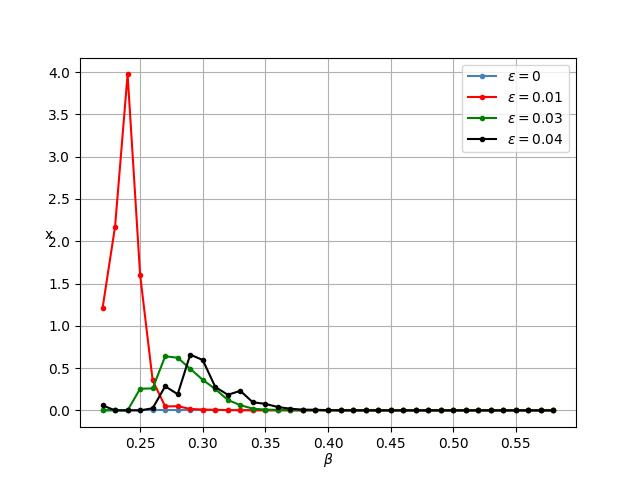
\includegraphics[width=\textwidth]{stochastic/variance_cyclic.jpg}
        
            \captionsetup{justification=centering}
            \caption{}
            \label{variance_cyclic}
        \end{figure}

    \subsection{Функция стохастический чувствительности}
    
        Функция стохастический чувствительности это инструмент, который показывает... 

        \comment{Думаю формулы тут не нужны, мб оставить ссылку на статью Crises, noise, and tipping in the Hassell population model}

        Давайте посмотрим на график \ref{bifurcation_x_0_2_a_1_beta_chaos_fss}. Красными линиями нарисована функция стохастический чувствительности. \comment{напиши зачем она тут вообще нужна}. 

        \begin{figure}
            \centering
            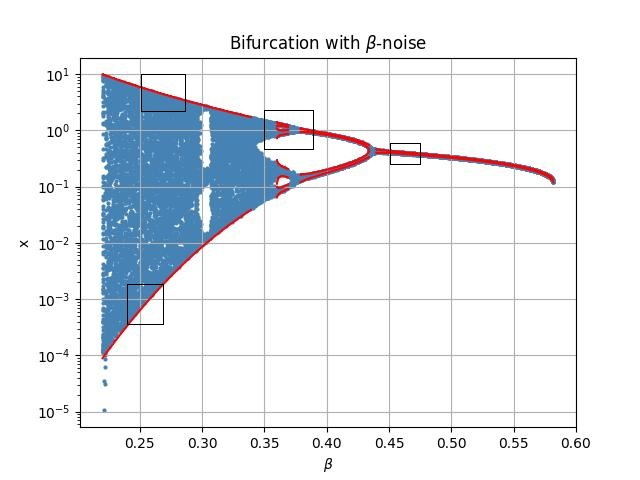
\includegraphics[width=\textwidth]{stochastic/bifurcation_x_0_2_a_1_beta_noise_fss.jpg}
        
            \captionsetup{justification=centering}
            \caption{График бифуркации с \(\beta\)-шумом.}
            \label{bifurcation_x_0_2_a_1_beta_chaos_fss}
        \end{figure}

        Рассмотрим участок от \(\beta \approx 0.45\) до \(\beta \approx 0.48\), он изображен на рисунке \ref{bifurcation_x_0_2_a_1_beta_chaos_fss_segment_stable}. Мы видим, что значения графика бифуркации почти всегда находятся в коридоре, границами которого являются значения ФСЧ. Этот коридор строится по правилу трех сигм. Такой подход гарантирует, что почти все значения будут находиться в этом интервале, что собственно мы и наблюдаем.

        \begin{figure}
            \centering
            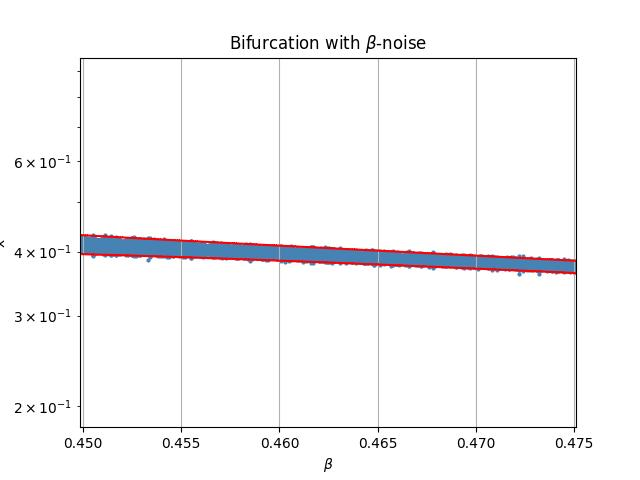
\includegraphics[width=\textwidth]{stochastic/bifurcation_x_0_2_a_1_beta_noise_fss_segment_stable.jpg}
        
            \captionsetup{justification=centering}
            \caption{}
            \label{bifurcation_x_0_2_a_1_beta_chaos_fss_segment_stable}
        \end{figure}

        На участках с k-циклами и хаосом (рисунки \ref{bifurcation_x_0_2_a_1_beta_chaos_fss_segment_2_cycle}, \ref{bifurcation_x_0_2_a_1_beta_chaos_fss_segment_chaos_up} и \ref{bifurcation_x_0_2_a_1_beta_chaos_fss_segment_chaos_down]}) будет наблюдаться аналогичная ситуация: значения лежат в коридоре, ограниченном значениями ФСЧ.

        \begin{figure}
            \centering
            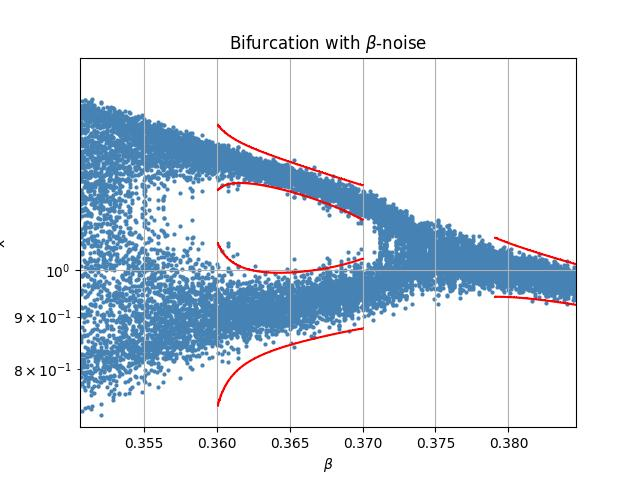
\includegraphics[width=\textwidth]{stochastic/bifurcation_x_0_2_a_1_beta_noise_fss_segment_2_cycle.jpg}
        
            \captionsetup{justification=centering}
            \caption{}
            \label{bifurcation_x_0_2_a_1_beta_chaos_fss_segment_2_cycle}
        \end{figure}

        \begin{figure}
            \centering
            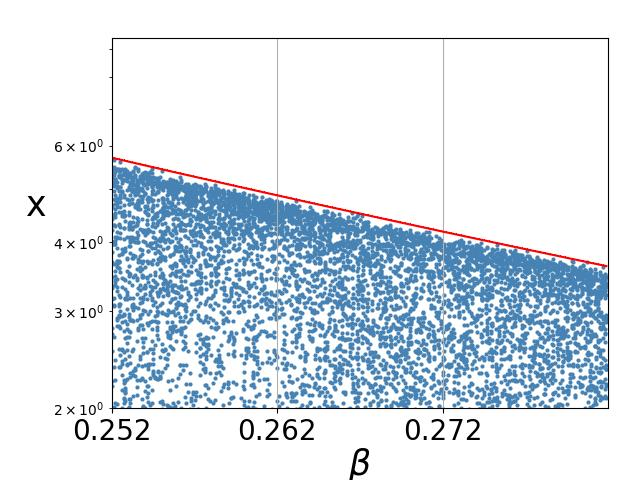
\includegraphics[width=\textwidth]{stochastic/bifurcation_x_0_2_a_1_beta_noise_fss_segment_chaos_up.jpg}
        
            \captionsetup{justification=centering}
            \caption{}
            \label{bifurcation_x_0_2_a_1_beta_chaos_fss_segment_chaos_up}
        \end{figure}

        \begin{figure}
            \centering
            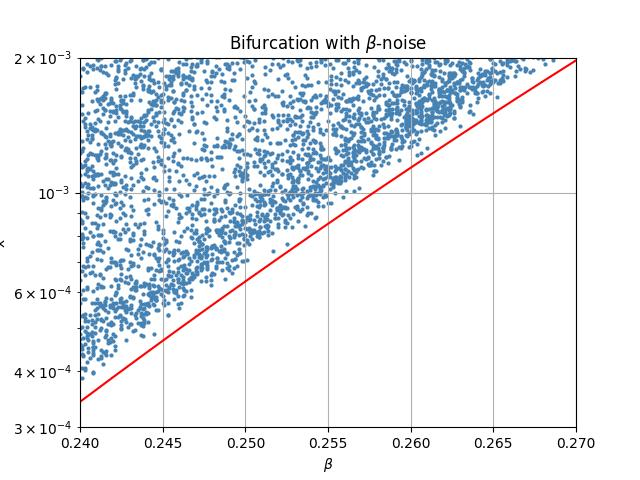
\includegraphics[width=\textwidth]{stochastic/bifurcation_x_0_2_a_1_beta_noise_fss_segment_chaos_down.jpg}
        
            \captionsetup{justification=centering}
            \caption{}
            \label{bifurcation_x_0_2_a_1_beta_chaos_fss_segment_chaos_down}
        \end{figure}

        \comment{напиши что-нибудь про ФСЧ}

    \subsection{График ФСЧ}

        Функцию стохастический чувствительности можно изобразить еще одним способом, который наглядно представлен на рисунках \ref{} \comment{которых пока нет.}

        \comment{напиши что-нибудь про график фсч, это который m(beta)}

    \subsection{Критическая интенсивность}

        Критической интенсивностью называется такое значение интенсивности, при котором траектории могут выходить за границы аттрактора и сваливаться в ноль.

        Например, на рисунке \ref{critical_intensity_beta_noise} изображен график критической интенсивности для \(\beta\)-шума. Красным показана критическая интенсивность для границ доверительных интервалов, которые лежат ниже устойчивого равновесия. Синим - для границ, которые выше устойчивого равновесия. 

        \comment{Наверное, не понятно про какие границы доверительного интервала идет речь}

        \comment{Для 4-цикла сделать шаг меньше и подойти ближе к 2-циклу. Холмик должен получится}

        \begin{figure}
            \centering
            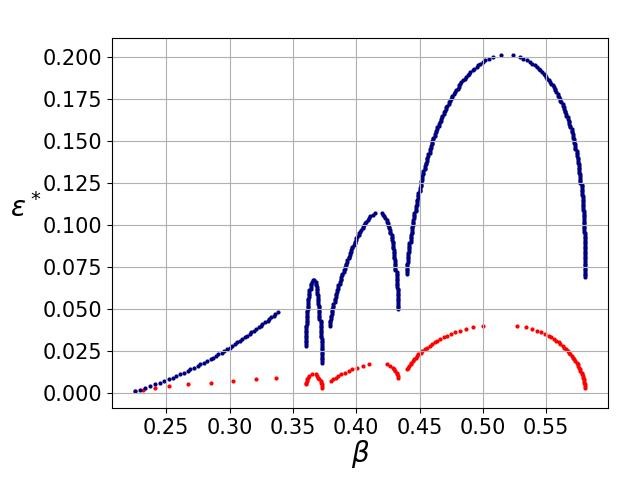
\includegraphics[width=\textwidth]{stochastic/critical_intensity_beta_noise.jpg}
        
            \captionsetup{justification=centering}
            \caption{}
            \label{critical_intensity_beta_noise}
        \end{figure}
        
        Обозначения аналогичны для графиков \(\alpha\)-шума (\ref{critical_intensity_alpha_noise}) и аддитивного шума (\ref{critical_intensity_additive_noise}).

        Интересно заметить, что в случае \(\alpha\)-шума и \(\beta\)-шума силуэты графиков очень похожи.

        \begin{figure}
            \centering
            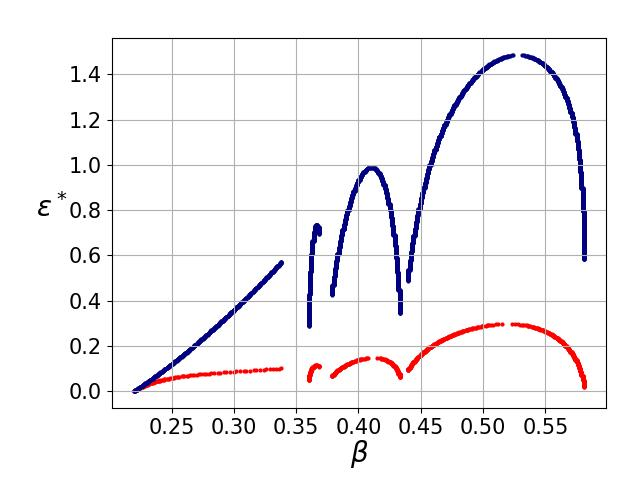
\includegraphics[width=\textwidth]{stochastic/critical_intensity_alpha_noise.jpg}
        
            \captionsetup{justification=centering}
            \caption{}
            \label{critical_intensity_alpha_noise}
        \end{figure}

        \begin{figure}
            \centering
            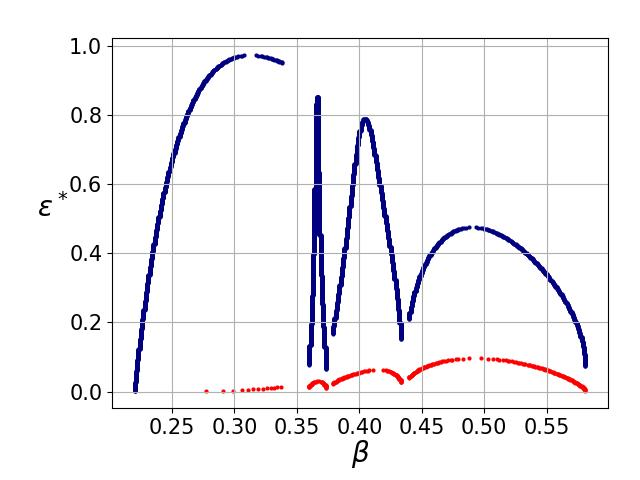
\includegraphics[width=\textwidth]{stochastic/critical_intensity_additive_noise.jpg}
        
            \captionsetup{justification=centering}
            \caption{}
            \label{critical_intensity_additive_noise}
        \end{figure}

        \comment{"Маловато будет!"}

    \subsection{Метрика Махаланобис}
        
        \comment{Тут опиши эту метрику}

        Метрика Махаланобис расчитывается по формуле 

        \[
            d_M = \frac{|x_1 - x^*|}{\sqrt{M}}
        \]
        
        где \(x_1\) --- устойчивое равновесие, \(x^*\) --- либо неустойчивое равновесие, либо его прообраз. \(M\) --- значение ФСЧ.

        Метрика Махаланобис показывает расстояние между двумя точками без учета того, что в модели \comment{что-то есть...}

        \comment{Ну и по традиции вставь картинки}

    \comment{Форматирование текста. Справа творится какая-то дчиь} 